\chapter{Method}

In this chapter we will describe the environment and motivation for our research. We will also explain the process for this study.

\section{Research Goal}
After over a decade of agile development where retrospectives have been recommended as a practice that should introduce improvements in development practices, the outcome of the retrospective is still undetermined. We will investigate this, focusing on the organizational learning that happens through retrospectives and the characteristics of the retrospective. When we say characteristics of the retrospective we will investigate the output of conducting retrospectives, the processes used and the impediments that faces the retrospective. We will investigate these characteristics in the context of existing academic work. \textit{Our goal for this study is to investigate the outcome returned from the retrospective in terms of organizational learning and retrospective characteristics.} Elaborating on this goal we get two sub-goals: 

\begin{enumerate}
	\item What are the main characteristics in current retrospective practices, in terms of outcome, processes and impediments? 
	\item How is learning achieved through current retrospective practices, in light of organizational learning theory? 
\end{enumerate}

The first sub-goal relates to the characteristics of the retrospective. We will throughout this study investigate and describe which characteristics are current in todays retrospective. We will focus on the output, the processes used and the impediments. When we say output we will investigate what improvement opportunities are created, which improvements are actually implemented and how the enthusiasm evolves as a result of the retrospective. We will also investigate the processes used by practitioners of the retrospective and the impediments that hinder them from returning value. 

The second sub-goal will investigate the learning achieved through the retrospective practice. We will employ the learning theory described by Argyris and Schön \cite{Argyris1996} and compare the governing values of Model I and Model II against the results we see from our case studies. We will also investigate which types of learning, single-, double-, or triple-loop, occur through the retrospective practice. 

\section{Research Design}
For this study we will conduct a multiple-case study to investigate our research goal. It will consist of one depth study and one breadth study. We describe each of these in short in this section and following in the chapter we will elaborate on these. A short summary of the research design can be seen in \autoref{table:research-design}. 

Our first case study is a depth study investigating the long-term practice of one retrospective practicing agile development team. This will be done through analyzing a set of retrospective reports using tabulations and then reflect on the results together with the team. 

The second case study is a breadth study investigating the retrospective practices of other teams. This will be done interviewing representatives from different retrospective practicing teams.

Our analysis method consists of two parts. The first part is a descriptive discussion on the results found during the two case studies that focuses on the characteristics of the retrospective practice. The second analysis method is comparing our results against the organizational learning framework created by Argyris and Schön \cite{Argyris1996} specifically the governing values of Model I and Model II. 

\begin{table}[!h]
	\begin{center}
	\caption{Research design for this multiple-case study.}
	\label{table:research-design}
	\makebox[\textwidth]{%
		\begin{tabular}{l p{0.7\textwidth}}
		\hline
		\textit{Step} & \textit{Description} \\
		\hline
		\textbf{Case 1} & Depth Study \\
		Content Analysis & Tabulation Analysis of Retrospective Reports \\
		Feedback Sessions & Reflection with team about the results of the content analysis. \\[12pt]
		\textbf{Case 2} & Breadth Study \\
		Interview Sessions & Interview different teams \\[12pt]
		\textbf{Analysis Method} & \\
		Characteristics & Descriptive Discussion on Results \\
		Organizational learning & Compare results against Argyris and Schön's \cite{Argyris1996} governing values. \\
		\hline
		\end{tabular}
	}
\end{center}
\end{table}

\section{Depth Study}
Our depth study consisted of two steps. The first step was to perform a content analysis on earlier retrospective reports. The second step was to hold several feedback sessions with the team reflecting on the results of the content analysis. We will describe each of these steps further in the following subsections.

\subsection{Content Analysis}

\subsubsection{Data Material - Retrospective Reports}
Through our supervisor we were put in contact with an experienced team in Norway. The team, which we will refer to as team Zulu is described more closely in \autoref{section:team-zulu-description}, graciously allowed us access to their retrospective logs, for us to analyze.

The retrospectives consisted of five different sections being: Where and What, Actions, Comments, Signatures and Case Proceedings, as can be seen in \autoref{table:retrospective-format}. 
The ``Where and What'' section contained general data about the retrospective such as the date, iteration dates, iteration number, contact person and other general information. ``Actions'' described the improvement actions that had resulted from the retrospective. It contained a description for each action, who is responsible for that action, deadline, status and comments from the participants. The ``Comments'' section contained comments, if any, from the participants of the retrospective if they had any specific input for the retrospective in general. ``Signatures'' contained the signature for each participant in the retrospective. The last section,``Case Proceedings'' contained information about the changes in the document and circulation of it.

\begin{table}[!h]
	\begin{center}
	\caption{The section of the retrospectives}
	\label{table:retrospective-format}
	\makebox[\textwidth]{%
		\begin{tabular}{l | p{0.7\textwidth}}
		\hline
		Part & Description \\
		\hline
		Where and What & Containing general data about the retrospective such as date, iteration location, etc. \\
		Actions & Describes the actions resulting from the retrospective it also includes data on responsible person, deadline etc. \\
		Comments & General comments from the participants for the retrospectives. \\
		Signatures & The signatures from each participant participating in the retrospective. \\
		Case Proceedings & The changelog and circulation of the retrospective. \\
		\hline
		\end{tabular}
	}
\end{center}
\end{table}

While getting familiar with the retrospectives we found that the only section containing any value in the terms of organizational learning was the actions described in the ``Action'' section. In most of the retrospective reports multiple actions were described relating to different issues observed during the iteration. The format of the actions can be seen in \autoref{table:action-format}. 

\begin{table}[!h]
	\begin{center}
	\caption{An generic example of an action provided in the retrospectives.}
	\label{table:action-format}
	\makebox[\textwidth]{%
		\begin{tabular}{| l  p{0.5\textwidth} |}
		\hline
		Action x &  \\
		Deadline & 01.01.2015 \\
		Action description & Always add a week to the iterations during holidays. \\
		Comments & Resources are not reliable during holidays. \\
		Responsible unit & Team X \\
		User responsible for action & John Smith \\
		Status & Completed or In Process \\
		Completed & 31.01.2014 \\
		Type & Preventive or Corrective \\
		\hline
		\end{tabular}
	}
\end{center}
\end{table}

\subsubsection{Analysis Method}
\label{analysis-method}
To retrieve any research-worthy knowledge from the actions given by the retrospective reports we needed means compare them. We settled on tabulations as our analysis method for the actions. Tabulations provide easy means of rendering data comprehensible. Krippendorff ~\cite{Krippendorff2004} describes tabulations as: 

\begin{quote}
Tabulation refers to collecting same or similar recording units in categories and presenting counts of how many instances are found in each. Tabulations produce tables of absolute frequencies, such as the number of words in each category occurring in a body of text, or of relative frequencies, such as percentages expressed relative to the sample size, proportions of a total, or probabilities.
\end{quote}

For our case we are going to use absolute frequencies to count the occurrences of different categories. Using relative frequencies would not suffice in our case where determining whether an action is twenty percent technical and eighty percent procedural or thirty percent technical and seventy percent procedural would be immensely difficult and not to mention impractical. Rather an action could be neither technical or procedural, be one of them, or be both. Thus resulting in us using absolute frequencies when we are counting occurrences of the different categories. 

To determine what the categories should be we conducted a pilot analysis that can be read about in Appendix \autoref{pilot-analysis}. The final result of categories were agreed upon by the team and are shown in \autoref{table:content-analysis-categories}. It consisted of six main themes: Nature, Context, Decision Making, Organizational Learning, Development and Collaboration. Nature, Context, Decision Making, Development and Collaboration can be related to the characteristics and output of retrospective practices. The organizational learning theme relates directly to the learning output and the team organizational learning of the practice. Each of the six themes had several categories which an action would be put in. These categories are shown in \autoref{table:content-analysis-categories} and are further described and defined in Appendix \autoref{appendix:categories}. 

\begin{table}[h]
	\begin{center}
		\caption{The final set of themes and categories that the content analysis is based upon.}
		\label{table:content-analysis-categories}
		\begin{adjustbox}{width=\textwidth, totalheight=0.9\textheight, keepaspectratio}
			\begin{tabular}{| l | l | p{0.5\textwidth} |}
			\hline
			Theme & Category & Short Description  \\
			\hline
			Nature & Positive & If an action is a result of a continuation of a process \\ \cline{2-3}
			& Negative & Action is a result of a arisen problem \\ \cline{2-3}
			& Undefined & The nature of the action is unclear or undefined \\ \hline
			Context & Technical & If the action is related to some technical context. \\ \cline{2-3}
			& Process & Action is related to a process context \\ \cline{2-3}
			& Undefined & The action could not be related to either technical or process \\ 
			\hline
			Decision Making & Strategic & Action is suggesting long-term change \\ \cline{2-3}
			& Tactical & The action is related to identification and use of resources. \\ \cline{2-3}
			& Operational & If the action is ensuring effectiveness and day-to-day operations \\ \cline{2-3}
			& Undefined & If the action is unclear and doesn't fit any of the other decision making categories. \\ 
			\hline 
			Organizational learning & Single-loop & If the action do a change that only influence the effects \\ \cline{2-3}
			& Double-loop & If one understand the factors that influence effects, and the nature of this influence. \\ \cline{2-3}
			& Undefined & If the action unclear in terms of organizational learning \\ \hline
			Development Phase & Development & Action is related to the development phase \\ \cline{2-3}
			& Testing & The action is related to testing \\ \cline{2-3}
			& Documentation & Action is related to Documentation \\ \cline{2-3}
			& Builds & The action is related to building of software systems \\ \cline{2-3}
			& Release & The action is related to releasing of software \\ \cline{2-3}
			& Business & The action is related to business development \\ \cline{2-3}
			& Undefined & The action is not related to any of the development phases described above \\ 
			\hline
			Collaboration & Communication & Related to communication within a team \\ \cline{2-3}
			& Leadership & Action is related to leadership \\ \cline{2-3}
			& Competence & Action is a result of lacking knowledge or experience \\ \cline{2-3}
			& External relations & The action is related to customer relations or other external stakeholders \\ \cline{2-3}
			& Planning & The action is a result of bad or good planning \\ \cline{2-3}
			& Undefined & Action is not related to any of the collaboration issues \\
			\hline
			\end{tabular}
		\end{adjustbox}
	\end{center}
\end{table}

In addition using tabulations for analyzing the actions, we investigated recurring issues. A retrospective is intended to highlight issues and potential actions that can be taken to correct or improve the issues. However it is not necessarily the case that every action is implemented as intended, or in the time frame originally intended. As such issues might come up again and again. Being able to identify these long term issues and address them before they become reoccurring is a clear potential improvement for a team or an organization. Therefore it is of great interest to identify these issues in our analysis. We will be looking through the available information and noting if an issue arises multiple times over time. Also of interest are unresolved issues, which are issues that are raised and a corrective action is agreed upon, but the action is either not implemented or implemented fully.

\paragraph{Processing Steps}
To perform our content analysis we first defined a set of processing steps that both authors were to follow. All the processing steps can be seen in \autoref{table:content-analysis-steps}.

\begin{table}
	\begin{centering}
		\caption{Description of the content analysis steps.}
		\label{table:content-analysis-steps}
		\begin{tabular}{l p{0.8\textwidth}}
			Step & Description \\ 
			\hline
			1 & Specify and document all the tabulation categories. \\
			2 & Send analysis documentation to the case participants to get feedback on the analysis measurements. \\
			3 & Create a spreadsheet for each author containing data on all the categories and all the actions. \\
			4 & Each author read through all the retrospectives separately, setting marks for each category that an action fits in. \\
			5 & When both authors were finished reading through all the retrospective they compared the results and put everything into a combined spreadsheet. If the authors disagreed on their markings a short discussion would commence and one would try to find an agreement. If an agreement could not be found the authors would turn to other external researchers to help identify the correct solution. \\
			6 & The content analysis was finished when all the actions were in the combined spreadsheet. \\
		\end{tabular}
	\end{centering}
\end{table}

The first step was to specify all the tabulation categories that were going to be included in the content analysis. Once all the categories were found and specified we documented them to ensure both authors had the same understanding of what each category meant. 

When the categories had been documented we sent them to the case participants to get feedback on the analysis measurements and verify that it was not anything that we had overlooked that the participants would like answers to. 

Once the feedback was incorporated into the content analysis we created a spreadsheet containing all the actions along the top row and all the categories along the first column. We created one spreadsheet for each author and one extra that would later be used for comparison. 

When the spreadsheets were done the next step was analyzing all the actions. Each author, separately, read through all the retrospectives and for each action marked which categories it belonged to. Each action could belong to several categories for an example an action could belong to both Testing and Documentation. For each of the six themes at least one mark had to be put down, and the maximum marks would be the number of categories in that theme. 

After all the retrospectives were read through and every action was tabulated the authors compared their results. For each action the authors would compare all the marks set for that action and if they both agreed upon all the marks the action would be copied to a new spreadsheet. If the authors disagreed they would go back to the action read it once more and try to find a classification that both could agree to. If this turned impossible we would seek advice from external researchers to gain a suitable solution. 

Once all the actions were compared and all the actions were in the new spreadsheet the content analysis was finished and data could then later be extracted from the spreadsheets. 
\afterpage{\clearpage}
\subsubsection{Content Analysis Limitations}
In this subsection we will describe the challenges and limitations of our content analysis from the 77 retrospectives. Mainly there were two challenges that occurred during our content analysis, missing contexts and borderline actions. Each is described in detail below. 
\paragraph{Missing Contexts}
As the retrospectives we were given mostly contained actions that resulted from the retrospective meetings, context of how the actions were brought to light could sometimes be missing. In those cases the actions either could have come from a problem happening during the iteration, a new idea that was put forth during the iteration or something similar. As some of the actions lacked context we included the undefined category to each theme so that in the cases were we could not tell whether an action was in a concrete development phase, or another theme, we could put it in undefined. 
\paragraph{Borderline Actions}
Borderline actions were the second challenge while performing our content analysis. An example is the action: 
\begin{quote}
To improve the understanding of the processes, the workflow diagrams and the other relevant documentation should be copied to the WIKI.
\end{quote}
This action could either be understood as ``The workflow diagrams and other relevant documentation is so good that we should put it on the WIKI'' or ``People do not have enough understanding of the processes and we should give them more documentation''. The first option could be classified as a positive action as the working documentation is good and should be used more, while the second option would be classified as a negative action as it is a problem that the understanding of the processes is not good enough. This action would be classified as undefined in our analysis as it both requires more context and as it lacks the context can be a borderline action between positive and negative. 

To deal with the borderline actions we added the steps of each author doing a separate analysis before comparing with the other author to identify the borderlines and find a adequate classification for them.

\subsection{Feedback Sessions}
As the final part of the first case-study several feedback sessions were held, to gather valuable input from the team and their reflections on the analysis. Each of these feedback session will be described in the following subsections. 

\subsubsection{Feedback Session: Team Discussion}
For the first feedback session we visited the team in person and held a presentation followed by a group discussion. The presentation was held in a meeting room in front of the team. The concept of the analysis was first explained and discussed with the team members, in order to ensure that there existed a common understanding of the work being presented. The presentation was also simultaneously a dialog between the presenters and the team. This was facilitated by constantly asking questions and encouraging discussion. One of the ways of encouraging discussion was to ask the team ``What expectations do you have for this category?'' before showing the results of the analysis. This ensured that we got their speculation as well as their reaction to the analysis. 

\subsubsection{Feedback Session: SCRUM Master Interview}
The second feedback session we had was an interview with the SCRUM master of the team. We spent a short while preparing and reviewing the questions we had prepared. The interview would be held in a semi-structured manner with the goal of having an open discussion of the results of the team discussion as well as gaining insight on the themes of the analysis. During the interview notes were taken, as well as recorded, and the SCRUM master was encouraged to speak his mind on relevant subjects. 

\subsubsection{Feedback Session: Team Leader}
The third feedback session was an interview where we presented additional findings, based on the results from the former feedback sessions and discussed the impact on the team. The interview was conducted with voice chat with the leader of the team. The session also served as a brainstorming session for the team leader in order to prepare a retrospective evaluation session he would lead the following week. This evaluation session would be a discussion between all members of the team where they discussed the current state of the retrospective after the feedback session and analysis.

\subsubsection{Feedback Session: Internal Team Evaluation}
The last session was conducted by the team internally without the authors present. The team had a ``Meta-Retrospective'' where they discussed the current state of the retrospective sessions, as well as their thoughts on the first feedback session. The team held the session as a normal retrospective, but with a semi-structured agenda that the team leader had developed in cooperation with the authors. The team leader then sent the meeting log to us, and had a short interview explaining the content.

\section{Breadth Study}
Our second case-study aimed to get a broader picture of the practices used for retrospectives today. We decided on a semi-structured interview, in order to be free to improvise as well as being prepared to ask stimulating questions to the interview subject.

\subsection{Semi-structured interviews}
We decided to use a semi-structured interview as our model for the interviews. An unstructured, or semi-structured does not have a complete script, and leaves room for improvisation, unlike a structured interview where there is a complete script. \cite{Myers2007} This approach was chosen to leave the interview subject free the elaborate on subjects they found interesting. 

A list of questions was prepared in order to serve as a guideline for the interview. This interview guide was divided into four sections, relevant for our research, being: ``General overview'', ``Team dynamics'', ``Organizational learning'' and ``Anything else''. A short description of each of these are shown in \autoref{table:interview-guide-overview}. The complete interview guide including all the questions can be found in appendix \autoref{section:interview-guide}. These four sections were chosen due to experiences working with team Zulu, as well as through a discussion with our supervisor. 

\begin{table}
	\begin{centering}
	\caption{Interview guide overview}
	\label{table:interview-guide-overview}
	\begin{tabular}{l p{0.8\textwidth}}
	 	Step & Description \\ 
		\hline
		General overview & Questions relating to the holding of the retrospective and learning\\
		Team dynamics & Questions on how team dynamics are handled and how they are experienced in the team \\
		Organization learning & Questions on how the team approach learning \\
		Anything else & Summary questions intended to cover potentially missed topics \\
	\end{tabular}
	\end{centering}
\end{table}

In order to conduct a successful semi-structured interview Myers and and Newman mentions several factors that need to be acknowledged \cite{Myers2007}. Among these are the lack of trust, elite bias and ambiguity of language. In order to avoid these potential pitfalls we spent time ensuring a mutual understanding and respect with the interview subject, for example by explaining our intentions and maintaining a friendly tone during the interview. 

The interviews were if possible held in person or over voice chat. This was done to lower the barrier for dialog as much as possible and let the interviewee speak as easily as possible. However at one point one interviewee had to resort to mail due to time constraints, we decided to keep the interview and the answers are included in the appendix. 

\subsection{Interview Subjects}
\label{subsec:Interview-Subjects}
In order to select interview subjects within the industry we contacted potential practitioners through e-mail or phone. As well as consulting our advisors. We wanted subjects with experience both holding and participating in retrospectives in order to gain multiple views of the retrospective experience. The base criteria was that participants had to be a part of a team that conducts retrospectives on a regular basis. We wanted a varied spread for the interview subjects and selected subjects based on their project and team compositions. Consultants, distributed teams, product development teams, small teams and big teams were some of the considerations for teams we wanted for this study.

\section{Analysis Method}
Our analysis method consisted of several steps. After gathering all the data from content analysis, feedback sessions and interviews each researcher went through the material separately. For the feedback sessions and interviews we listened through the recordings taking notes ensuring nothing was missed during the sessions. After all the material was worked through we compared the different data against each other and against earlier academic work. The academic fields used is: Retrospective literature and organizational learning. The fields was chosen as retrospectives is a shared learning activity and thus organizational learning is useful to see how the team as a whole learns and retrospective literature  as it can be used to compare the characteristics for retrospective practices.

\begin{figure}[!h]
	\centering
	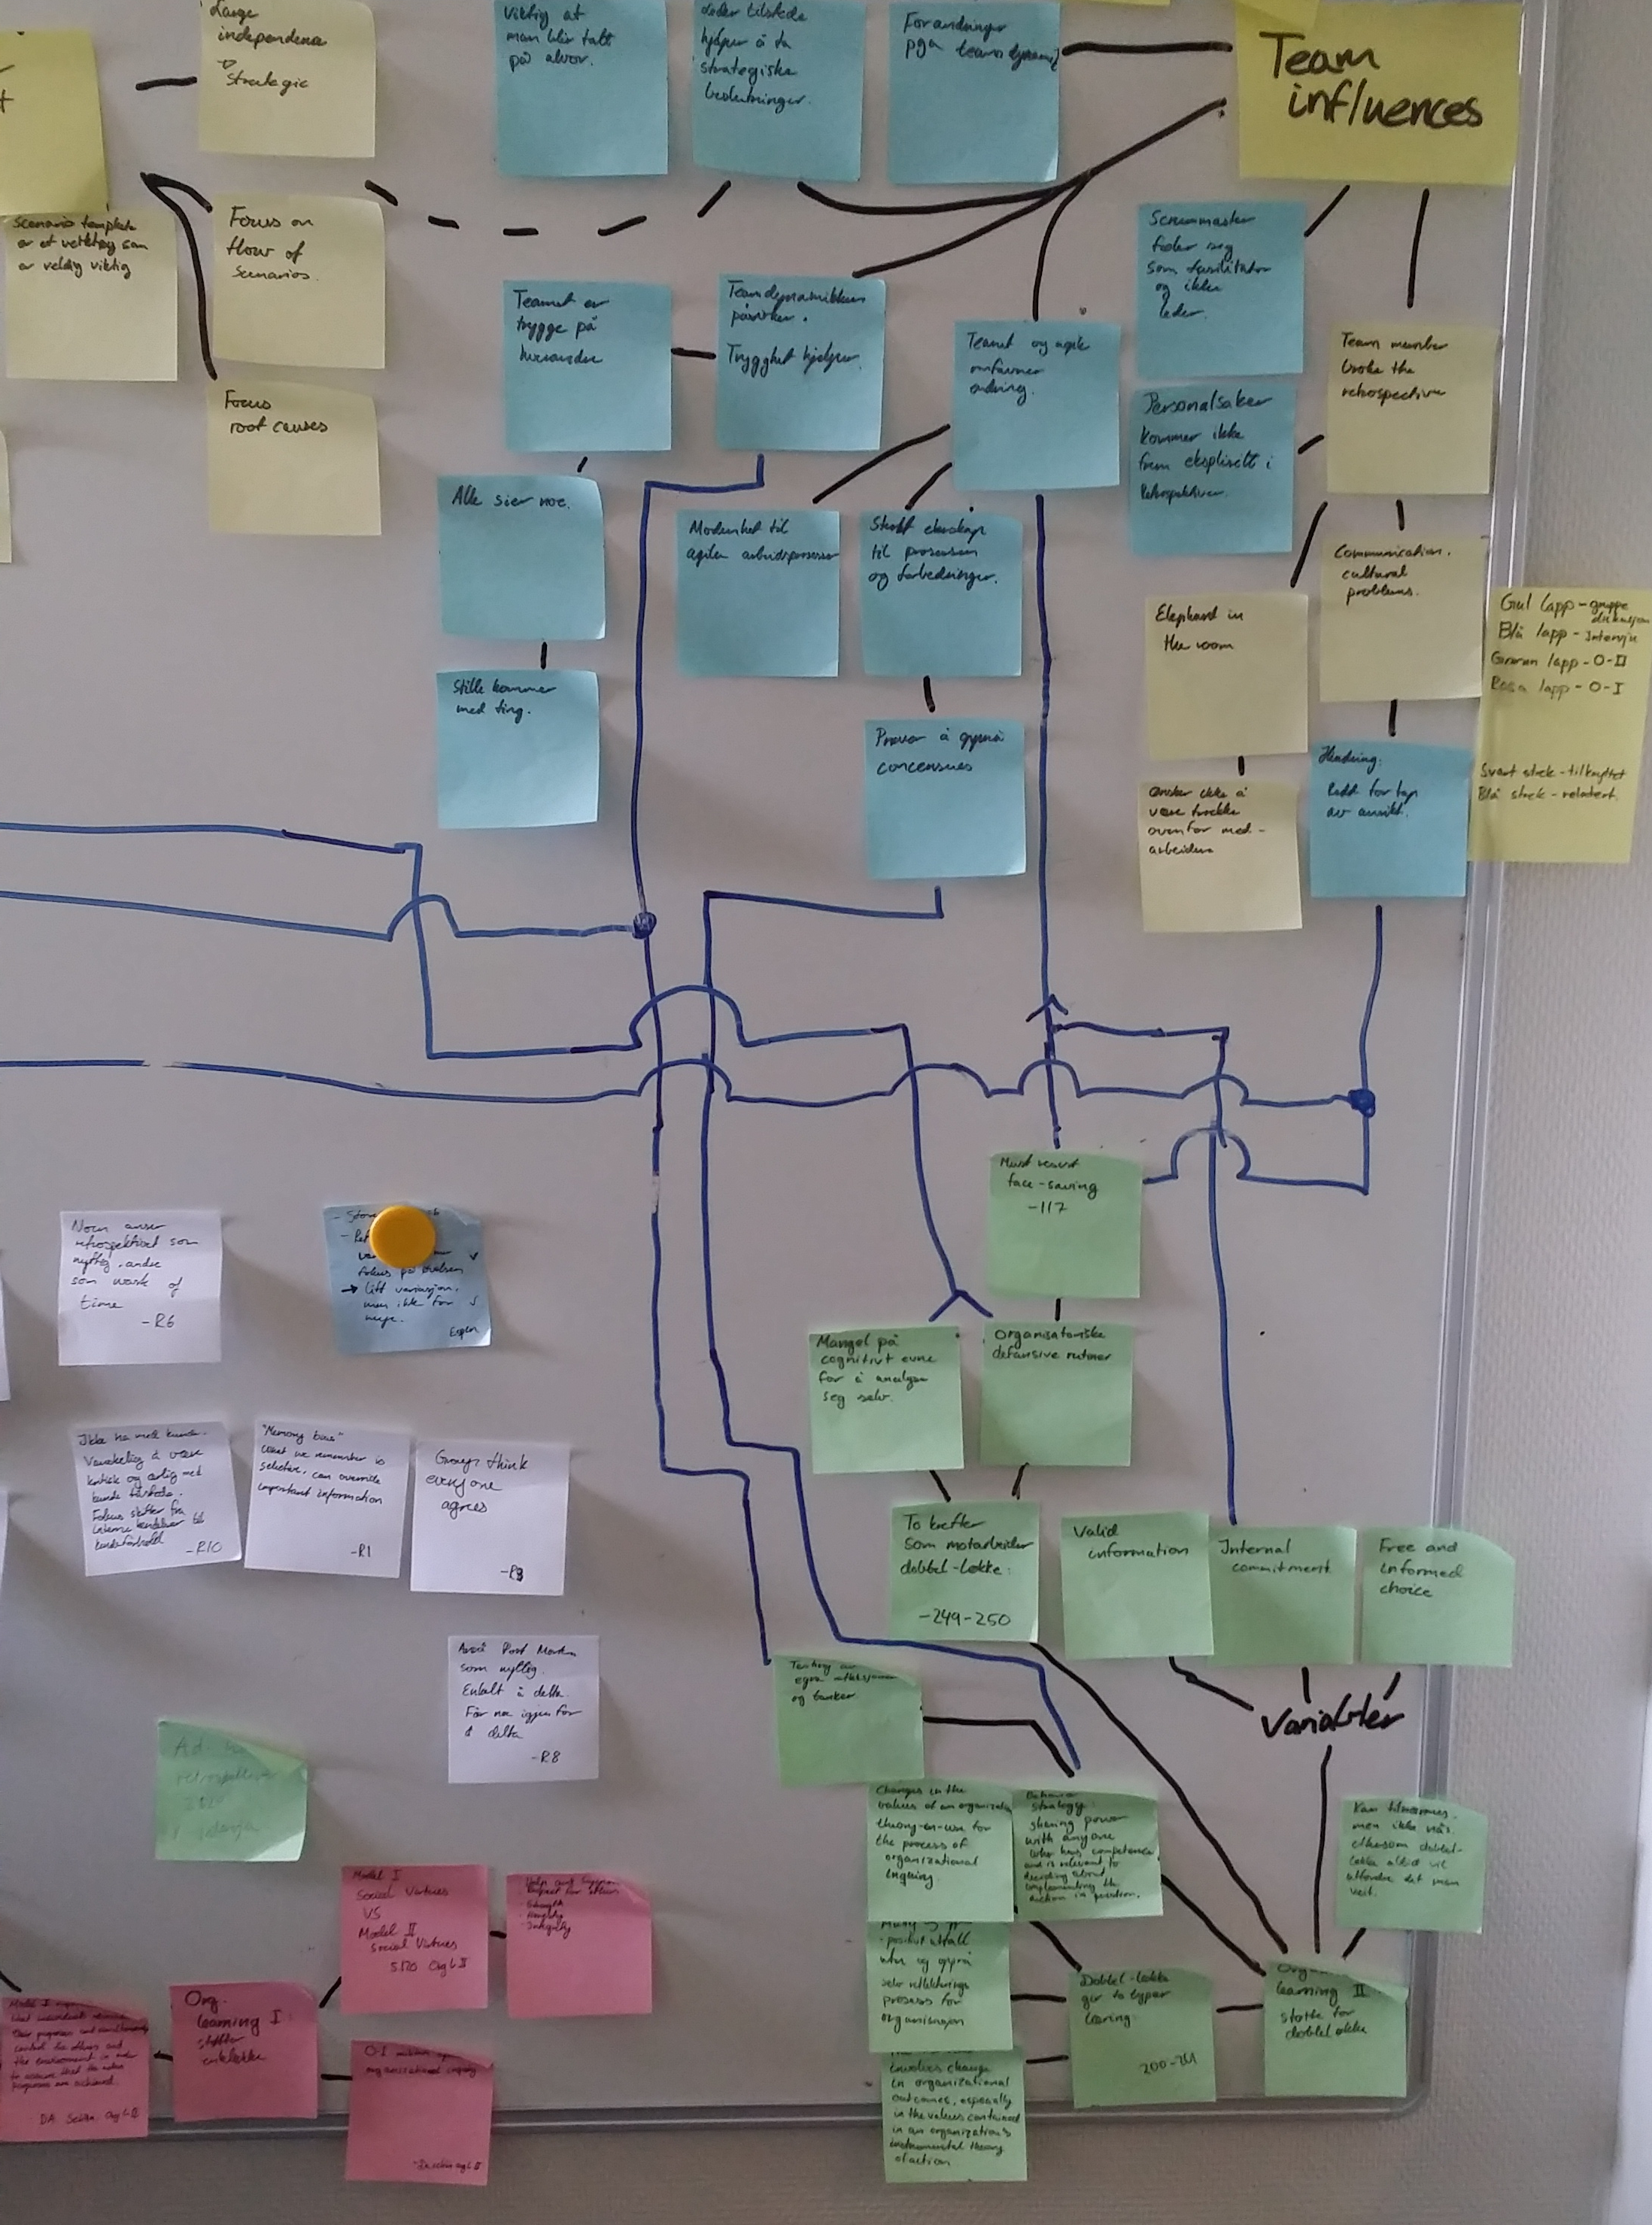
\includegraphics[height=0.5\textheight, keepaspectratio]{figures/analysis.png}
	\caption{A picture of our whiteboard during analysis}
	\label{fig:Analysis-trends}
\end{figure}

\clearpage

\section{Participants}
Our research bases itself on the primary data gathering methods: Retrospective depth analysis of one team and interview input from other teams. In this section we will present the participants using the phonetic alphabet as identifiers. Many of the participants were recruited from existing research projects being ``Agile 2.0'' and ``SMIGLO''.

\subsection{Depth Analysis Participant - Team Zulu}
\label{section:team-zulu-description}
Team Zulu is situated in Norway and develop a human resource system. The team has been working with agile principles for over 10 years. An overview of the team can be seen in \autoref{list:team-zulu}

 \begin{enumerate}
 \label{list:team-zulu}
	\item 1 HoD – Product Owner 
	\item 1 SCRUM Master
	\item 1 Architect
	\item 4 Developers
	\item 1 Content Responsible
	\item 2 Testers
	\item 1 Build and DB responsible
	\item 1 Third line support engineer
\end{enumerate} 

\subsection{Breadth Study Participants}
In this section it is a short description of each interview subject. All participants in the interview research were familiar with retrospectives, and agile development practices. The selection process is described in \autoref{subsec:Interview-Subjects} and an overview of the team and representatives can be found in \autoref{table:participants}

\subsubsection{Team Alfa}
Team Alfa consisted of 22 members and we spoke to two of them. The project leader and one developer. The team consisted of designers, testers, front-end developers and back-end developers who all worked with media solutions for a customer. 

\subsubsection{Team Bravo}
Team Bravo consisted of 6 members, 2 in Norway, 3 developers in Poland and 1 tester in Shanghai. The project leader and Scrum master were in Norway. 

\subsubsection{Team Charlie}
From team Charlie we spoke to one representative. The participant was project coordinator, project leader and SCRUM master for a development team consisting of four persons. The participant also had responsibility for agile practices in his company which develops HR solutions. 

\subsubsection{Team Delta}
The representative for Team Delta was a developer and the teams SCRUM master. The team developed HR solutions. 

\subsubsection{Team Echo}
The participant from team Echo was a consultant acting as a developer and semi-project leader for a multi-platform development project. The team consisted of 10 members and developed four different products for one customer.

\subsubsection{Team Foxtrot}
Team Foxtrot consisted of about 20 members in the roles of design, ux, front-end, back-end and project leaders. The representative from team Foxtrot was a system developer and he chose to responded to our interview through email. We acknowledge that this might have a resulted in input getting lost. However the input that has been gathered will still be able to give us some data which can be used for this study. 

\subsubsection{Team Golf}
Team Golf consisted of 2 members working in Norway, with the rest of the team situated in Shanghai. The representative from Team Golf was the SCRUM master for the team. 

\begin{table}[!h]
	\begin{center}
	\caption{Table overview over interview participants}
	\label{table:participants}
	\begin{tabular}{l p{0.5\textwidth} l}
	\hline
	Team & Description & eRpresentatives\\
	\hline
	Alfa & Project leader & 2 \\
	& Developer & \\
	Bravo & SCRUM Master & 1  \\
	Charlie & SCRUM master, project leader and coordinator & 1 \\
	Delta & Developer and SCRUM master & 1 \\
	Echo & Developer and project leader & 1 \\
	Foxtrot & System Developer & 1 \\
	Golf & SCRUM Master & 1 \\
	\hline
	\end{tabular}
	\end{center}
\end{table}

\clearpage